\section{Dataset and exploratory data analysis}
\label{sec:eda}

\subsection{The Credit Risk Dataset}
The dataset \cite{kaggle_credit} has \num{32581} rows and 12 columns: seven numeric features, four categorical features and the binary target (\cref{tab:overview}).
The dataset is released under CC0 (public domain).
The notebook downloads it from a public mirror in the project's GitHub releases, falls back to Kaggle, and verifies its SHA-256 checksum, so every run uses exactly the same file.

\begin{table}[H]
  \centering
  \small
  \begin{tabularx}{\linewidth}{lX}
    \toprule
    \textbf{Column} & \textbf{Meaning} \\
    \midrule
    \ident{person_age} & Age of the applicant (years) \\
    \ident{person_income} & Annual income (USD) \\
    \ident{person_home_ownership} & RENT, MORTGAGE, OWN or OTHER \\
    \ident{person_emp_length} & Employment length (years) \\
    \ident{loan_intent} & Purpose: EDUCATION, MEDICAL, VENTURE, PERSONAL, DEBTCONSOLIDATION, HOMEIMPROVEMENT \\
    \ident{loan_grade} & Lender's risk grade from A (best) to G (worst) \\
    \ident{loan_amnt} & Requested amount (USD) \\
    \ident{loan_int_rate} & Interest rate (\%) \\
    \ident{loan_percent_income} & Loan amount divided by annual income \\
    \ident{cb_person_default_on_file} & Whether the credit bureau records a past default (Y/N) \\
    \ident{cb_person_cred_hist_length} & Length of the credit history (years) \\
    \ident{loan_status} & \textbf{Target}: 1 = default, 0 = non-default \\
    \bottomrule
  \end{tabularx}
  \caption{Columns of the Credit Risk Dataset.}
  \label{tab:columns}
\end{table}

\begin{table}[H]
\centering
\small
\begin{adjustbox}{max width=\linewidth}
\begin{tabular}{llrrr}
\toprule
column & type & missing & missing (\%) & unique \\
\midrule
person\_age & numeric & 0 & 0.00 & 58 \\
person\_income & numeric & 0 & 0.00 & 4295 \\
person\_home\_ownership & categorical & 0 & 0.00 & 4 \\
person\_emp\_length & numeric & 895 & 2.75 & 36 \\
loan\_intent & categorical & 0 & 0.00 & 6 \\
loan\_grade & categorical & 0 & 0.00 & 7 \\
loan\_amnt & numeric & 0 & 0.00 & 753 \\
loan\_int\_rate & numeric & 3116 & 9.56 & 348 \\
loan\_status & categorical & 0 & 0.00 & 2 \\
loan\_percent\_income & numeric & 0 & 0.00 & 77 \\
cb\_person\_default\_on\_file & categorical & 0 & 0.00 & 2 \\
cb\_person\_cred\_hist\_length & numeric & 0 & 0.00 & 29 \\
\bottomrule
\end{tabular}
\end{adjustbox}
\caption{Columns of the raw dataset.}
\label{tab:overview}
\end{table}


\subsection{Data quality}
\label{subsec:quality}

\paragraph{Duplicates.}
\num{165} rows are exact duplicates of other rows.
They are removed, because duplicates inflate the apparent sample size and can land on both sides of the train/test split.

\paragraph{Impossible values.}
Five applicants are older than 100 (two of them are 144), and two report 123 years of employment while being 21 and 22 years old (\cref{fig:boxplots}).
These are data-entry errors, not genuine extremes.
We turn them into missing values, using the rules age $> 100$ and employment length $>$ age $-$ 14, and let the imputer fill them.
The rules are deterministic and row-local, so applying them before the split cannot leak information.

\begin{figure}[H]
  \centering
  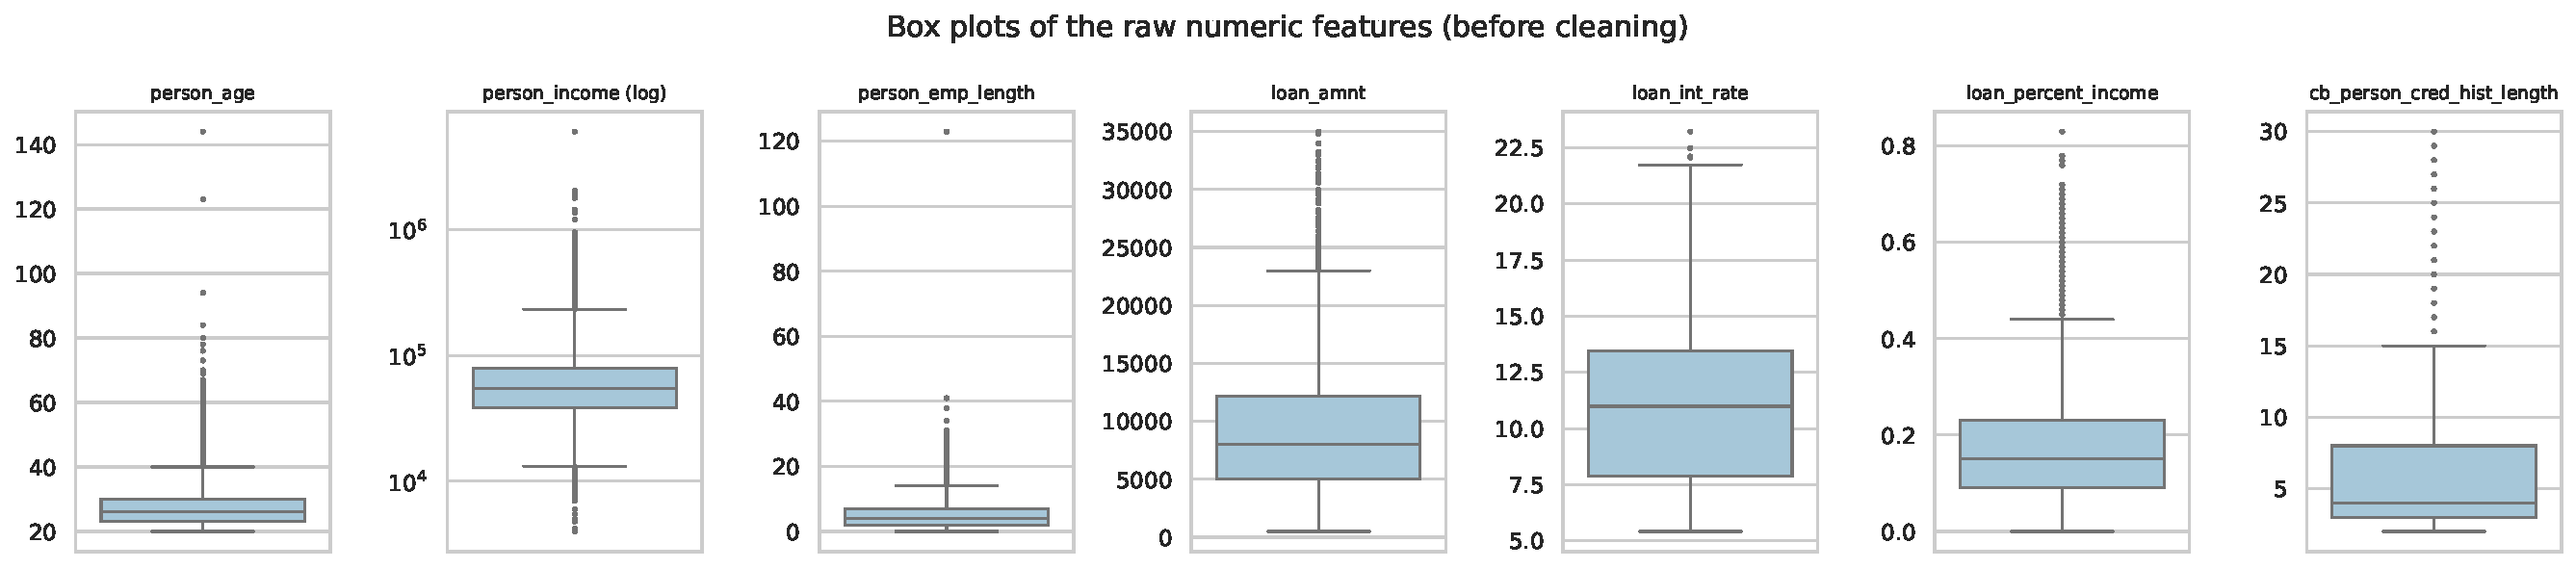
\includegraphics[width=\linewidth]{eda_boxplots.pdf}
  \caption{Box plots of the raw numeric features. Note the impossible ages and employment lengths, and the heavy right tails of income and amounts.}
  \label{fig:boxplots}
\end{figure}

\paragraph{Skewness and genuine outliers.}
Income is extremely right-skewed (skewness 32.9, median \$55{,}000, maximum \$6{,}000{,}000).
The loan amount, loan-to-income ratio and credit-history length also have long right tails.
Unlike the impossible values, these are plausible and are kept.
Whether to winsorize them or log-transform them is treated as a pipeline option and decided experimentally (\cref{tab:suite_outlier_fe}).

\begin{table}[H]
\centering
\scriptsize
\begin{adjustbox}{max width=\linewidth}
\begin{tabular}{lrrrrrrrr}
\toprule
feature & mean & std & min & 1\% & 50\% & 99\% & max & skew \\
\midrule
person\_age & 27.73 & 6.35 & 20.00 & 21.00 & 26.00 & 50.00 & 144.00 & 2.58 \\
person\_income & 66074.85 & 61983.12 & 4000.00 & 14400.00 & 55000.00 & 225200.00 & 6000000.00 & 32.87 \\
person\_emp\_length & 4.79 & 4.14 & 0.00 & 0.00 & 4.00 & 18.00 & 123.00 & 2.61 \\
loan\_amnt & 9589.37 & 6322.09 & 500.00 & 1000.00 & 8000.00 & 29800.00 & 35000.00 & 1.19 \\
loan\_int\_rate & 11.01 & 3.24 & 5.42 & 5.42 & 10.99 & 18.62 & 23.22 & 0.21 \\
loan\_percent\_income & 0.17 & 0.11 & 0.00 & 0.02 & 0.15 & 0.50 & 0.83 & 1.06 \\
cb\_person\_cred\_hist\_length & 5.80 & 4.06 & 2.00 & 2.00 & 4.00 & 17.00 & 30.00 & 1.66 \\
\bottomrule
\end{tabular}
\end{adjustbox}
\caption{Descriptive statistics of the numeric features (raw data).}
\label{tab:numeric}
\end{table}


\subsection{Target distribution}
Only 21.8\% of the loans defaulted (\cref{fig:target}).
This moderate imbalance drives three design decisions:
\begin{itemize}[nosep]
  \item the split and every cross-validation fold are stratified;
  \item accuracy is not used for model selection, PR-AUC and F2 are used instead (\cref{subsec:protocol});
  \item class weights, SMOTE and under-sampling are compared as remedies.
\end{itemize}

\begin{figure}[H]
  \centering
  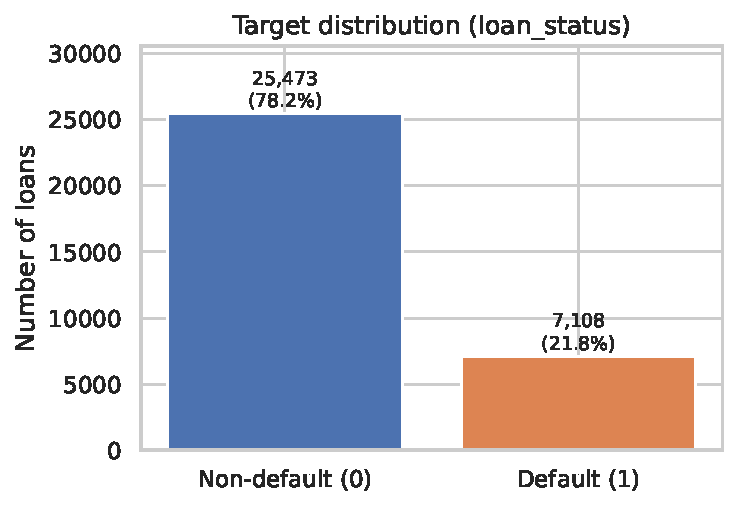
\includegraphics[width=0.5\linewidth]{eda_target.pdf}
  \caption{Distribution of the target \ident{loan_status}.}
  \label{fig:target}
\end{figure}

\subsection{Numeric features}
\Cref{fig:numeric} compares the class-conditional distributions after cleaning.
Three features separate the classes clearly.
\begin{itemize}[nosep]
  \item \ident{loan_percent_income}: defaulters typically borrow more than 30\% of their income, while most non-defaulters stay below 20\%.
  \item \ident{loan_int_rate}: defaulters concentrate at rates above 14\%.
  \item \ident{person_income}: defaulters have lower incomes (on the log scale).
\end{itemize}
Age, employment length and credit-history length have nearly identical distributions in both classes.
Most applicants are young (median age 26; 76\% are 30 or younger).

\begin{figure}[H]
  \centering
  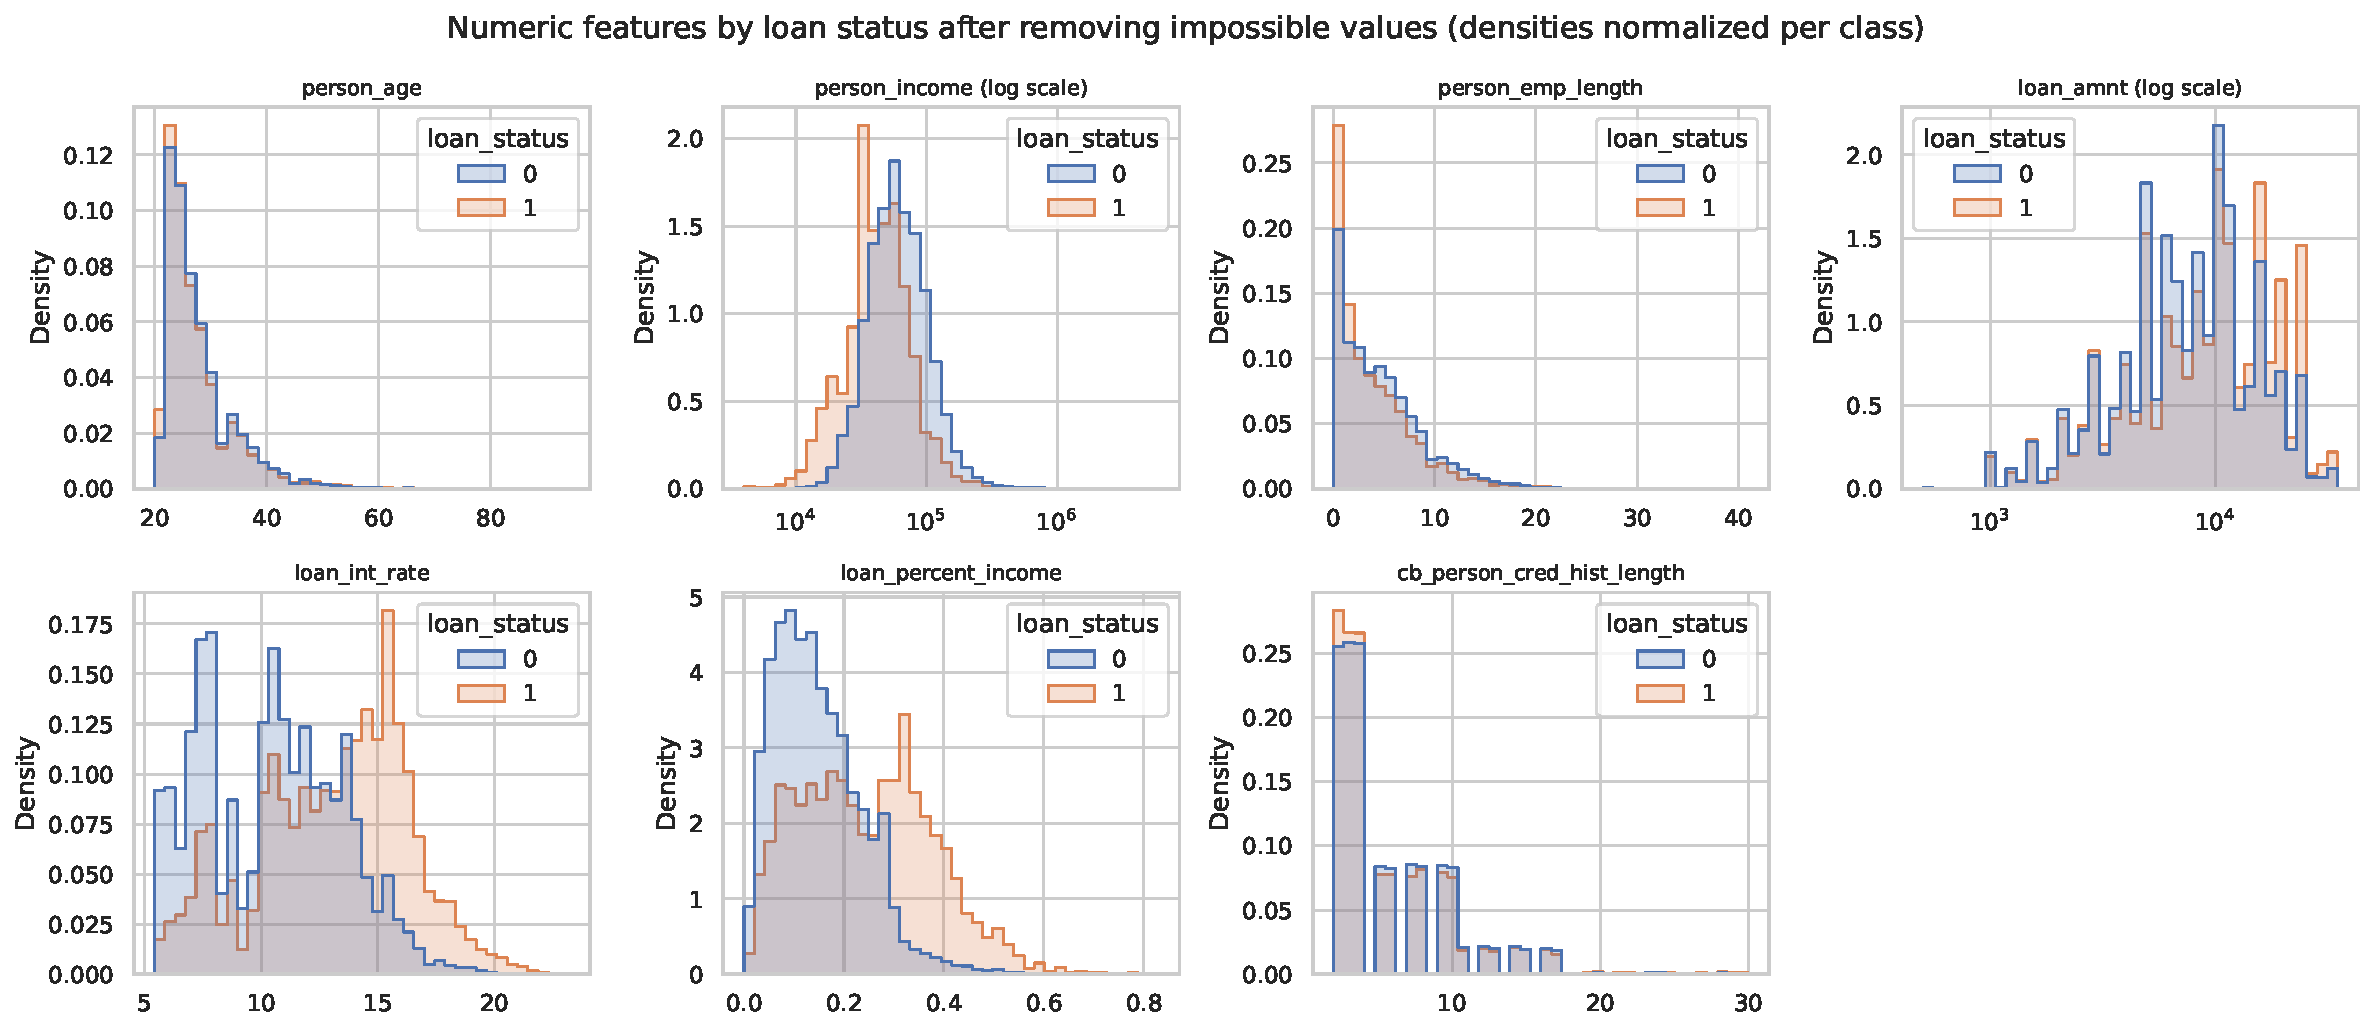
\includegraphics[width=\linewidth]{eda_numeric.pdf}
  \caption{Class-conditional distributions of the numeric features (after removing impossible values; densities normalized per class).}
  \label{fig:numeric}
\end{figure}

\subsection{Categorical features}
\Cref{fig:categorical} shows the frequency of each category and its default rate.
\begin{itemize}[nosep]
  \item \textbf{Loan grade} is the strongest categorical signal. The default rate rises monotonically from 10.0\% (A) and 16.3\% (B) to 59.0\% (D) and 98.4\% (G). The jump between C and D is the largest. The order supports an ordinal encoding.
  \item \textbf{Home ownership}: renters default four times as often as owners (31.6\% versus 7.5\%). Mortgage holders sit in between (12.6\%). The OTHER category is rare (107 rows).
  \item \textbf{Past default on file}: 37.8\% of applicants with a recorded past default default again, against 18.4\% of the others.
  \item \textbf{Loan intent} has a weaker effect, from 14.8\% (VENTURE) to 28.6\% (DEBTCONSOLIDATION).
\end{itemize}

\begin{figure}[H]
  \centering
  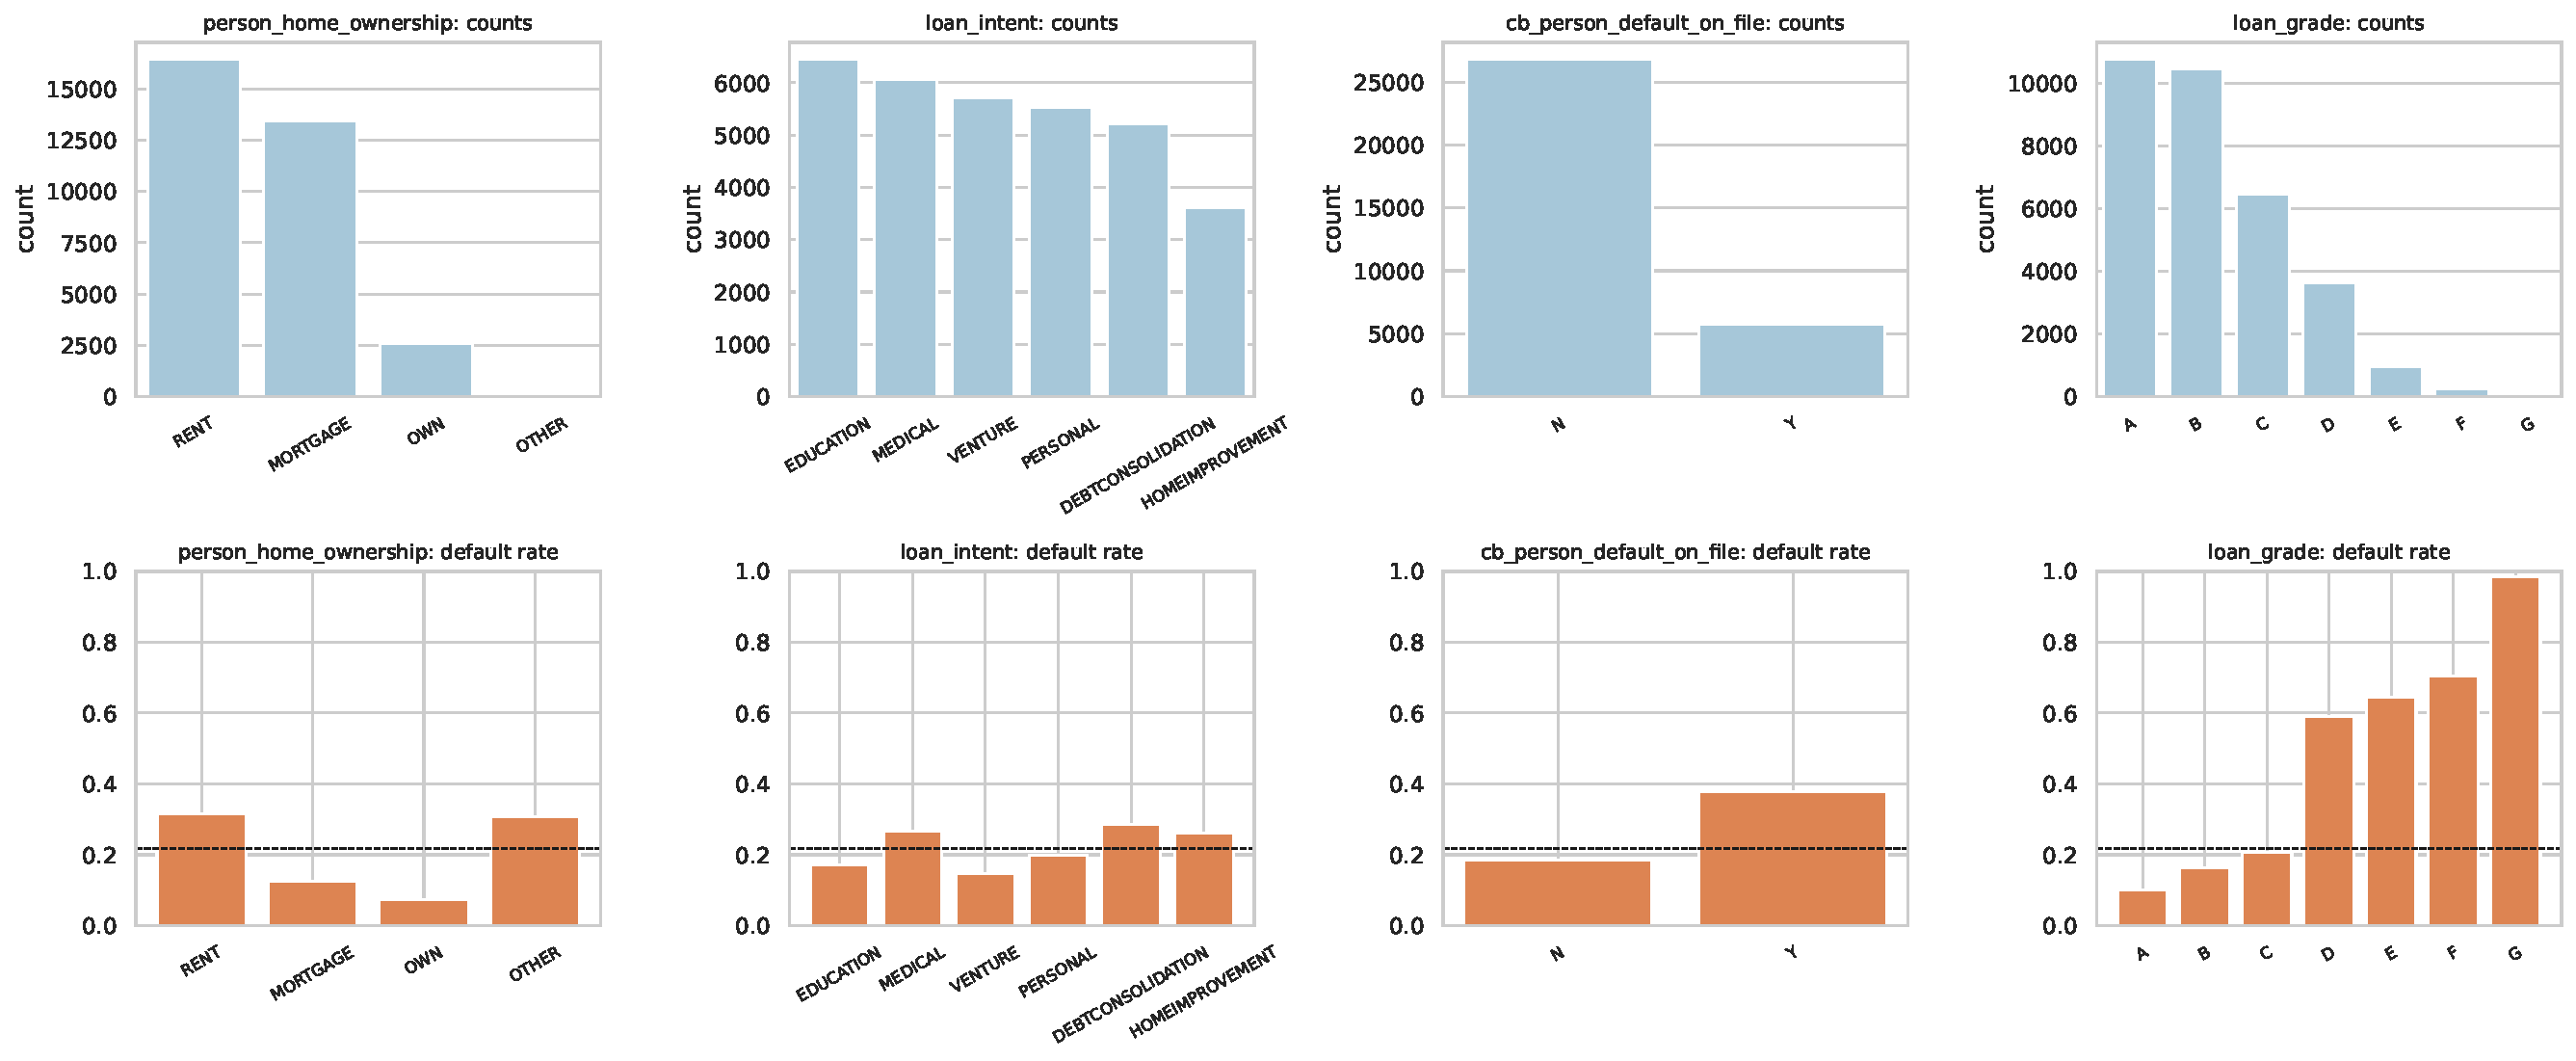
\includegraphics[width=\linewidth]{eda_categorical.pdf}
  \caption{Categorical features: counts (top) and default rate per category (bottom; the dashed line is the overall rate).}
  \label{fig:categorical}
\end{figure}

\subsection{Correlations and feature relevance}
The Spearman correlation matrix (\cref{fig:correlation}) reveals three strongly related pairs:
\begin{itemize}[nosep]
  \item the interest rate and the grade ($\rho = 0.95$): the lender prices loans by grade;
  \item age and credit-history length ($\rho = 0.81$);
  \item the loan amount and the loan-to-income ratio ($\rho = 0.65$).
\end{itemize}
These redundancies matter for linear models (collinearity), and they explain why a single grade-related feature carries most of the signal.
The features most correlated with the target are the grade (0.33), the interest rate (0.32), the loan-to-income ratio (0.32) and the income ($-0.27$).

Mutual information (\cref{fig:mi}) also captures non-monotone dependence.
It ranks income first, followed by the loan-to-income ratio, the grade and the interest rate.
Age and credit-history length carry almost no information on their own.
The scatter plot in \cref{fig:burden} shows that the classes overlap strongly in any single feature, but that defaults concentrate where low income meets a high loan-to-income ratio.
This is an interaction that tree ensembles can capture directly.

\begin{figure}[H]
  \centering
  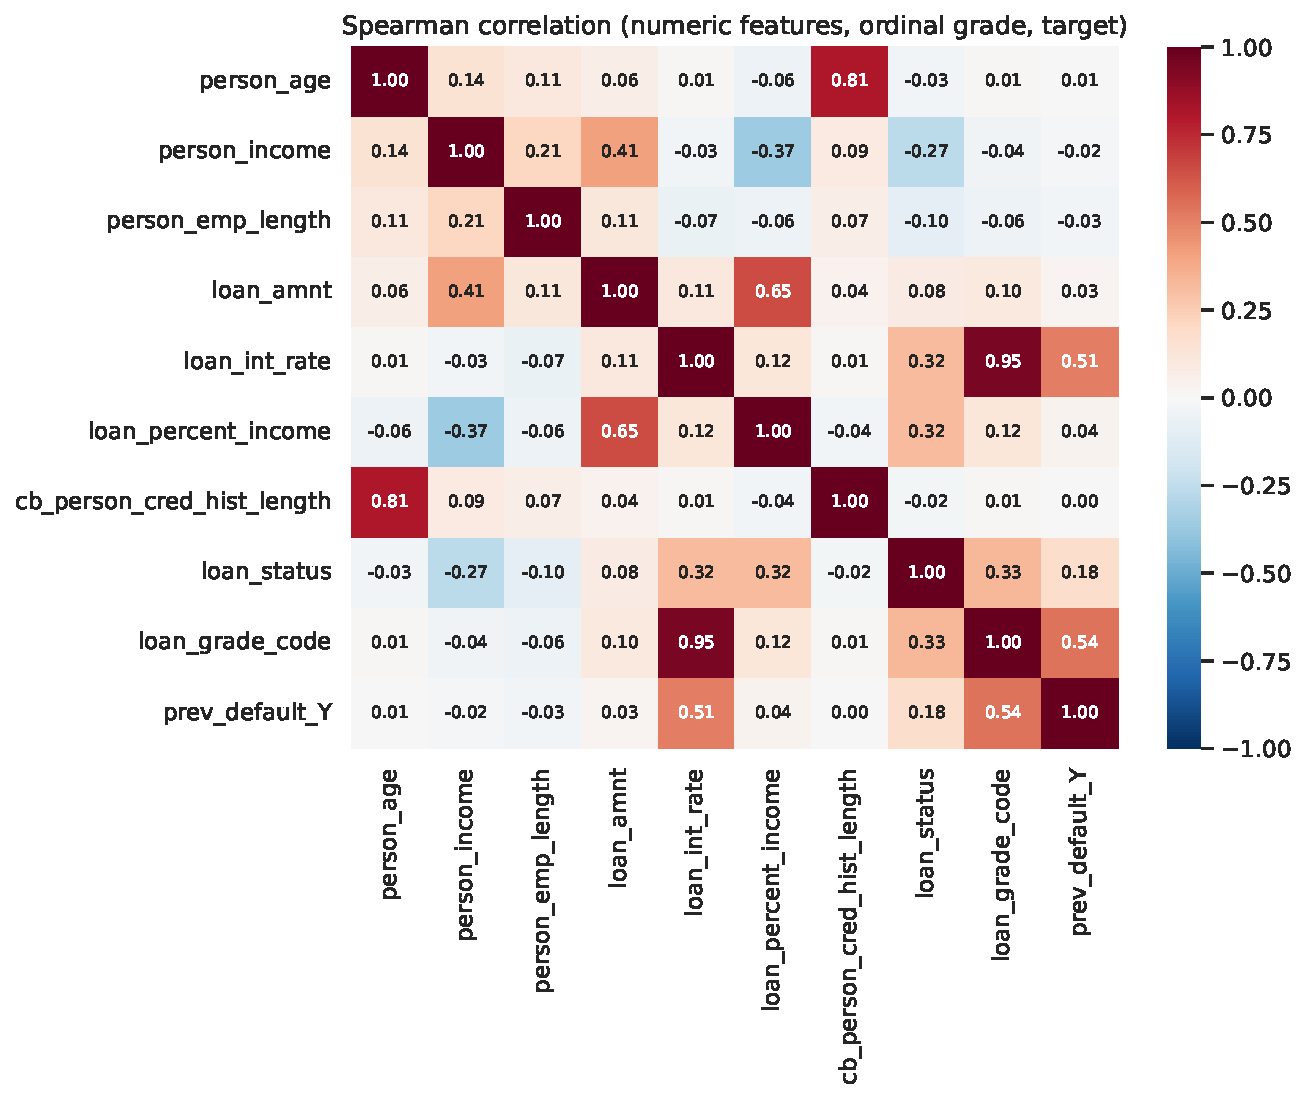
\includegraphics[width=0.75\linewidth]{eda_correlation.pdf}
  \caption{Spearman correlations between numeric features, the ordinal grade, the past-default flag and the target.}
  \label{fig:correlation}
\end{figure}

\begin{figure}[H]
  \centering
  \begin{subfigure}{0.49\linewidth}
    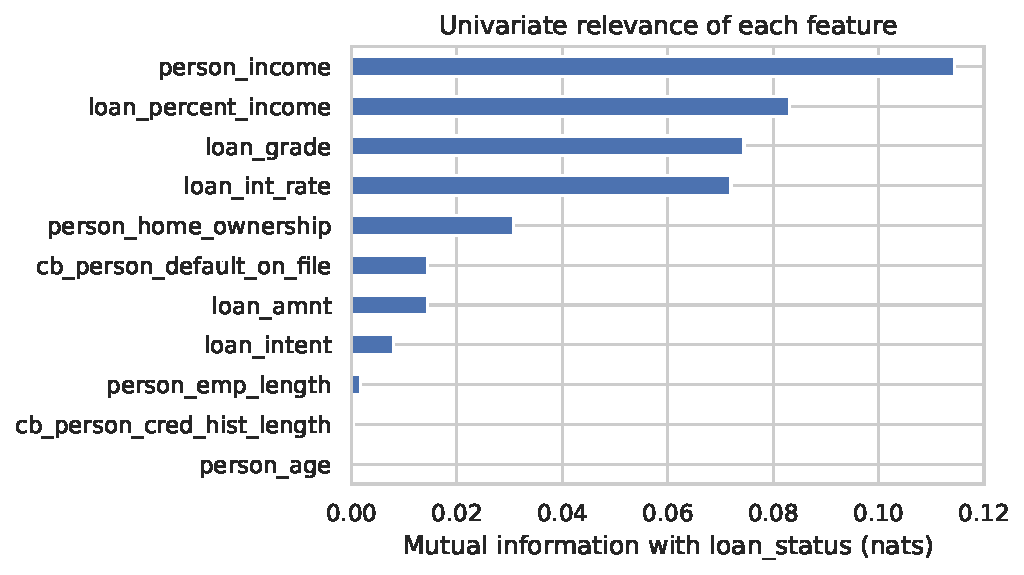
\includegraphics[width=\linewidth]{eda_mutual_info.pdf}
    \caption{Mutual information with the target.}
    \label{fig:mi}
  \end{subfigure}
  \hfill
  \begin{subfigure}{0.49\linewidth}
    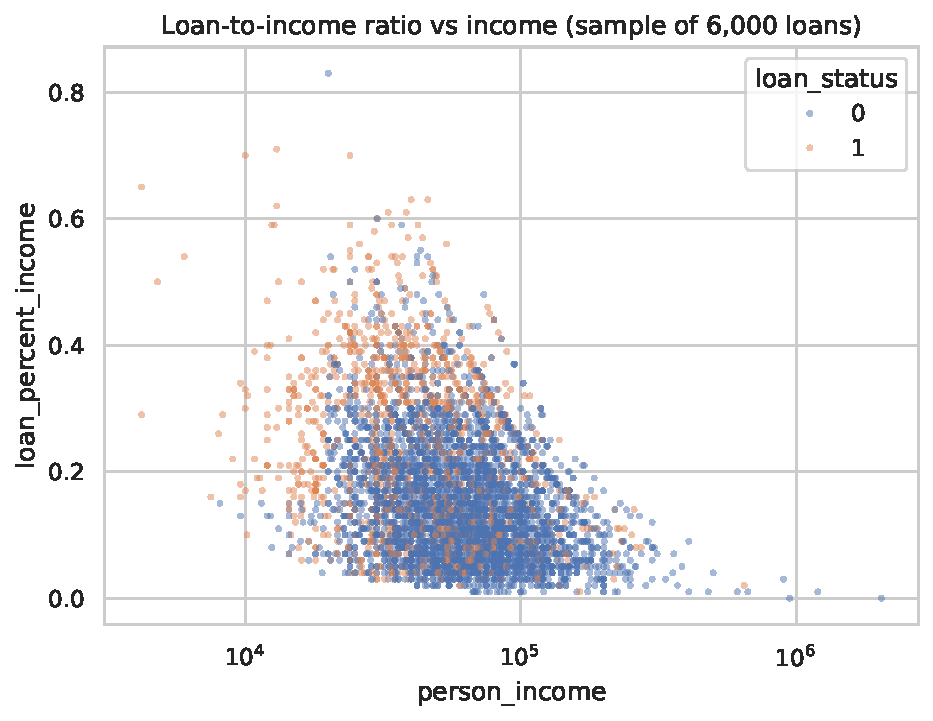
\includegraphics[width=\linewidth]{eda_burden.pdf}
    \caption{Loan-to-income ratio versus income.}
    \label{fig:burden}
  \end{subfigure}
  \caption{Relevance of individual features and an example interaction.}
\end{figure}

\subsection{Missing values}
\label{subsec:missing}
Two columns have missing values: \ident{person_emp_length} (895 rows, 2.75\%) and \ident{loan_int_rate} (\num{3116} rows, 9.56\%).
They are missing together in only 68 rows.
\Cref{fig:missing} shows that the two columns behave differently.
\begin{itemize}
  \item A missing \textbf{interest rate} is uninformative. Loans with a missing rate default at 20.7\%, against 21.9\% for loans with an observed rate, and the share of missing rates is flat across grades. This is consistent with \emph{missing completely at random}. Because the rate is almost determined by the grade (\cref{fig:rate_grade}), the grade-wise median is a natural imputation.
  \item A missing \textbf{employment length} is informative. These applicants default at 31.5\%, against 21.5\% otherwise. The missingness itself carries signal, which motivates the optional missing-value indicators.
\end{itemize}

\begin{figure}[H]
  \centering
  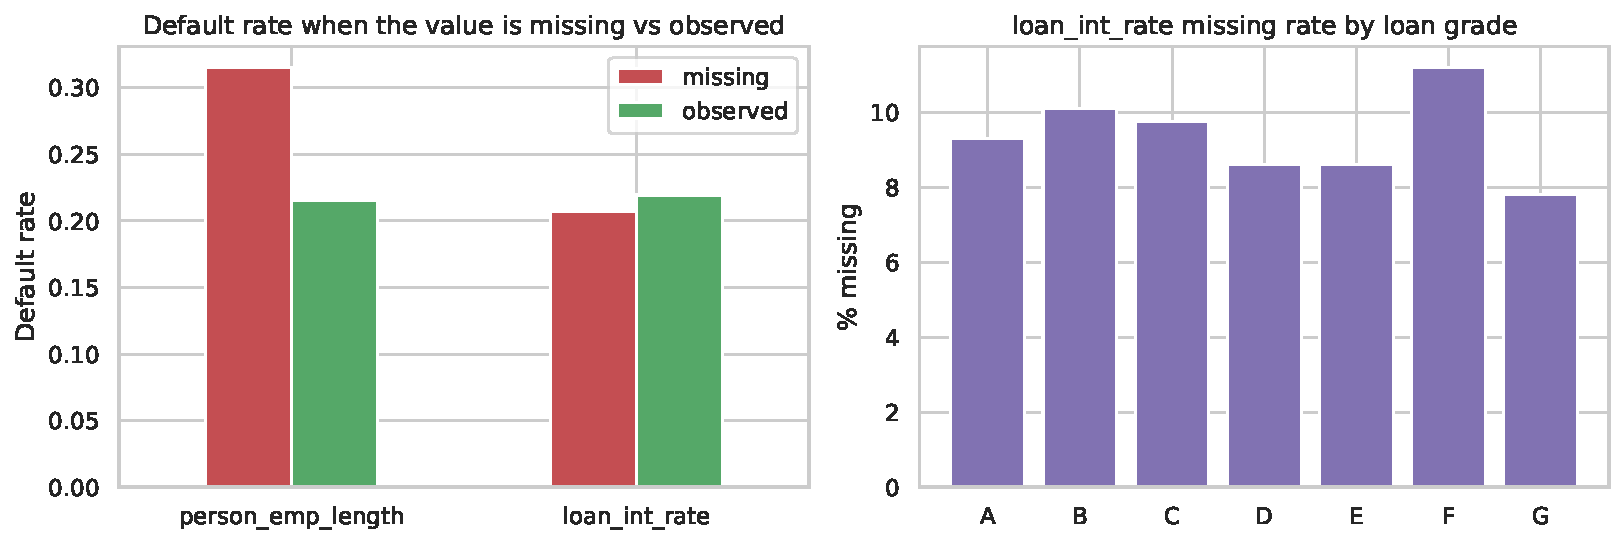
\includegraphics[width=\linewidth]{eda_missing.pdf}
  \caption{Left: default rate when a value is missing or observed. Right: missing share of \ident{loan_int_rate} per grade.}
  \label{fig:missing}
\end{figure}

\begin{figure}[H]
  \centering
  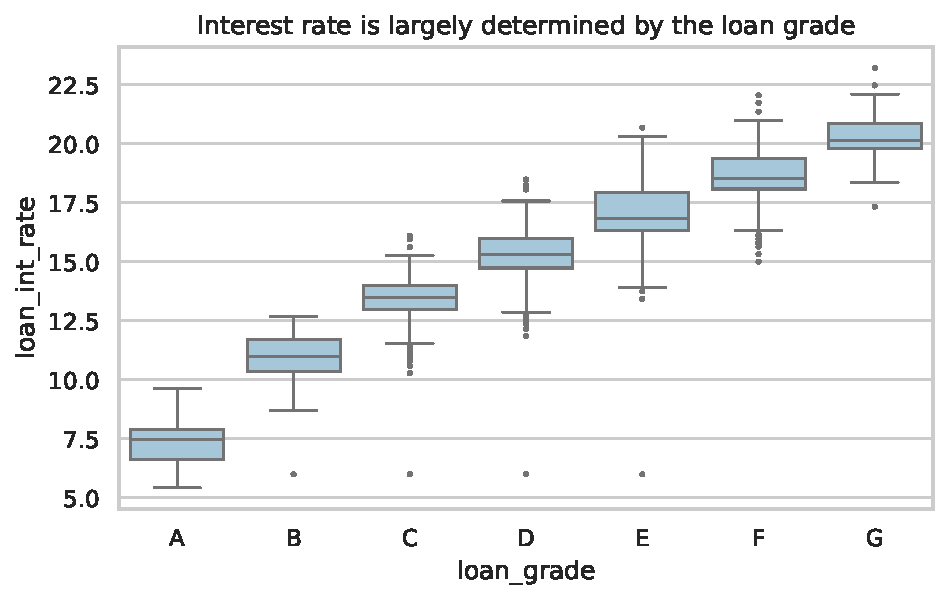
\includegraphics[width=0.6\linewidth]{eda_rate_grade.pdf}
  \caption{Interest rate by loan grade: the grade almost determines the rate.}
  \label{fig:rate_grade}
\end{figure}

\subsection{Implications for the pipeline}
\Cref{tab:eda_decisions} summarizes how the findings shape the pipeline.

\begin{table}[H]
  \centering
  \small
  \begin{tabularx}{\linewidth}{XX}
    \toprule
    \textbf{Finding} & \textbf{Pipeline decision} \\
    \midrule
    165 duplicates, 7 impossible values & Rule-based cleaning before the split; impossible values become missing \\
    21.8\% defaults, asymmetric error costs & Stratification; PR-AUC for selection and an F2-tuned threshold; class-imbalance remedies compared \\
    Interest rate determined by grade & Grade-wise median imputation as an option \\
    Informative missing employment length & Optional missing-value indicators \\
    Heavy right tails (income, amounts) & IQR winsorizing or log transform as options; log features in feature engineering \\
    Monotone default rate across grades & Ordinal versus one-hot grade encoding compared \\
    Very different scales (income vs ratios) & Scaler choice compared, essential for k-NN and SVM \\
    Correlated features, only 11 inputs & PCA and feature selection tested, with little redundancy expected \\
    Interactions (income $\times$ burden, grade $\times$ housing) & Tree ensembles and neural networks expected to do well \\
    \bottomrule
  \end{tabularx}
  \caption{From EDA findings to pipeline options.}
  \label{tab:eda_decisions}
\end{table}
